\chapterOrPart{Making drawings and plots}\label{ch:drawing}
This chapter contains some examples of figures and charts. More will be added in the future.

It's possible to make all kinds of drawings in \LaTeX\ with the package \pkg{TikZ}. The style of objects can be predefined. See for instance the source code for \cref{fig:3systems} where the blue fill colour and the red dashed border of the three systems are defined with the command \cs{tikzstyle} in the style file \verb|styles/myDrawingStuff|.

\section{Simple \TikZ\ drawing}

\begin{frame}{An example of a drawing that uses properties that are defined on the document level}
    \begin{figure}[htbp]\centering
		\begin{tikzpicture}
            % see styles/myDrawingStuff.sty for global definitions of: system, mass and heat
            % this means that you can use them in other drawings too
    		%\draw [help lines] (0,0) grid (10,4); % uncomment to show a grid
    		\draw [system] (0,0) ellipse (1.5cm and 1cm) node [black]{open};
    		\draw [system] (4,0) ellipse (1.5cm and 1cm) node [black]{closed};
    		\draw [system] (8,0) ellipse (1.5cm and 1cm) node [black]{isolated};
    		\draw [mass] [<->] (0,0.75) -- + (0,0.5) node [above] {mass};
    		\draw [heat] [<->] (0,-0.75) -- + (0,-0.5) node [below] {energy};
    		\draw [heat] [<->] (4,-0.75) -- + (0,-0.5) node [below] {energy};
		\end{tikzpicture}
    	\caption{Mass and energy transfer in thermodynamic systems, to illustrate the use of \texttt{tikzstyle} for defining object properties}\label{fig:3systems}
    \end{figure}
\end{frame}

\section{Drawing block diagrams}
It's possible to draw block diagrams in \TikZ, as for example in \cref{fig:flowchart}. In this figure, the properties of the blocks and connectors are defined globally in \verb|styles/myDrawingStuff|, so that they can also be used in other diagrams in the document.

\begin{figure}\centering
    \begin{tikzpicture}[auto, node distance=0.6cm and 1.5cm]
        % see styles/myDrawingStuff for block diagram styles used in this figure
     
        % place blocks
        \node [model]                      (hydraulic) {hydraulic\\ model};
        \node [block, right = of hydraulic](pressure)  {pressure losses};
        \node [block, below = of pressure] (pumping)   {pumping work};
        \node [block, below = of pumping]  (elec)      {electricity};
        \node [kpi,   right = of elec]     (LCOE)      {LCOE};
        \node [kpi,   below = of LCOE]     (CO2)       {\ch{CO2eq}};
        \node [block, right = of LCOE]     (gas)       {gas};
        \node [block, above = of gas]      (heat)      {heat demand};
        \node [model, above = of heat]     (thermal)   {thermal\\ model};

        % draw arrows
        \draw [connectline] (hydraulic) -- (pressure);
        \draw [connectline] (pressure)  -- (pumping);
        \draw [connectline] (pumping)   -- (elec);
        \draw [connectline] (elec)      -- (LCOE);
        \draw [connectline] (thermal)   -- (heat);
        \draw [connectline] (heat)      -- (gas);
        \draw [connectline] (gas)       -- (LCOE);
        \draw [connectline] (gas)       |- (CO2);
        \draw [connectline] (elec)      |- (CO2);
    \end{tikzpicture}
	\caption{Block diagram drawn in \TikZ, to illustrate the use of drawing styles and connectors}\label{fig:flowchart}
\end{figure}

Another type of block diagram, a process control scheme, is shown in \cref{fig:control}. The original source code for \cref{fig:control} can be found on \href{www.texample.net/tikz/examples/control-system-principles}{TeXample.net}, built by \textcite{texample} and was adapted in this template.

\begin{figure}\centering
    \begin{tikzpicture}[auto, node distance=2.5cm,>=latex']
        %\draw [helpline] (0,2) grid (10,-3);
        \tikzstyle{block}   = [draw, fill=green!20, rectangle, minimum height=3em, minimum width=6em]
        \tikzstyle{sum}     = [draw, fill=green!20, circle, node distance=1cm]
        \tikzstyle{input}   = [coordinate]
        \tikzstyle{output}  = [coordinate]
        
        % place blocks
        \node [input, name=input] {};
        \node [sum, right of=input] (sum) {};
        \node [block, right of=sum] (controller) {controller};
        \node [block, right of=controller,node distance=4cm] (system) {system};
        
        % position the node u between the controller and system block
        % we can then position the measurement block below the node u
        \draw [->]                      (controller) -- node[name=u] {$u$} (system);
        \node [block, below of=u]       (measurements) {measurements};
        \node [output, right of=system] (output)       {};
    
        % draw arrows
        \draw [draw,->] (input)        -- node[pos=0.2] {$i$} node[pos=0.8] {$+$} (sum);
        \draw [->]      (sum)          -- node {$e$} (controller);
        \draw [->]      (system)       -- node [name=y] {$y$}(output);
        \draw [->]      (y)            |- (measurements);
        \draw [->]      (measurements) -| node[pos=0.90] {$-$} node [near end] {$y_\up{m}$} (sum);
        \draw [<-]      (system.north) --  +(0,0.4) node[above] {$\delta$};
    \end{tikzpicture}
	\caption{Example of a system control diagram drawn in \TikZ}\label{fig:control}
\end{figure}

\section{Process flow diagram}\label{sec:processflowdiagram}
Process flow diagrams (PFDs) can be drawn with the help of the \pkg{pfdicons} package. An example of a PFD of a Rankine cycle is shown in \cref{fig:steamcycle}. See also \cref{sec:pfdicons}.

\begin{figure}[h]\centering
% adapted from p. 19 of ctan.tetaneutral.net/graphics/pgf/contrib/pfdicons/pfdicons-doc.pdf
    \begin{tikzpicture}[node distance=3cm]	
		% components
		\node [basic hx,         scale=1.5, rotate=90] (boiler) {};
		\node [turbine,          scale=2.0, below right= of boiler] (turbine) {};
		\node [basic hx,         scale=1.5, rotate=90, below left= of turbine] (cond) {};
		\node [centrifugal pump, scale=1.0, below left=of boiler, unit int=inlet south, unit ext=outlet north west] (pump) {};

  		% tags
		\node[below]  at (boiler.west)  {boiler};
		\node[above]  at (cond.east)    {condenser};
		\node[left]   at (turbine.west) {turbine};
  		\node[right]  at (pump.east)    {pump};
    
		% mass flows
		\draw[blue,->] (boiler.south) -| (turbine.nnw);
		\draw[blue,->] (turbine.sse)  |- (cond.south);
		\draw[blue,->] (cond.north)   -| (pump.center);
		\draw[blue,->] (pump.outlet)  |- (boiler.north);
		
        % energy flows (styles 'heat, cold, work' are defined in styles/myDrawingStuff}
		\draw[heat,<-] (boiler.east)  -- node[pos=1.5] {$\dot{Q}_\up{in}$} ++(0,5mm);
		\draw[cold,->] (cond.west)    -- node[pos=1.5] {$\dot{Q}_\up{out}$} ++(0,-5mm);
		\draw[work,->] (turbine.east) -- node[pos=2.0] {$\dot{W}_\up{turb}$} ++(5mm,0);
		\draw[work,<-] (pump.west)    -- node[pos=2.0] {$\dot{W}_\up{pump}$} ++(-5mm,0);
	\end{tikzpicture}
    \caption{Process flow diagram of a Rankine cycle \parencite[adapted from][p.~19]{pfdicons}, to illustrate the capacity of the package \pkg{pfdicons} to draw PFDs}\label{fig:steamcycle}
\end{figure}

\section{Extracting a specific region from a PDF file}
It's easy to extract a specific rectangular region from a PDF file while preserving the image quality in vector format. This is useful for incorporating figures and tables from publications into your work without sacrificing image quality, as often happens when resorting to screenshots. This method is illustrated in \cref{fig:partofpdf} where a specific figure from a certain page of a PDF file is included twice. The left figure is included with the command \cmd{includegraphics} with the desired \cmd{page} and \cmd{trim} values, combined with the option \cmd{clip}. By doing so, the vector format will be retained. Consequently, the figure remains sharp, even when scaled up for placement on a poster. The right figure is a screenshot of the same region. As you can see, its resolution is limited, making it less suited for magnification and placement on a poster. You can verify this by zooming in on the two figures.
\begin{figure}\centering
    % trim margins: left bottom right top 
    \includegraphics[page={3},trim={2cm 21.7cm 6cm 2.7cm}, clip,width=0.49\textwidth]{figs/T100.pdf}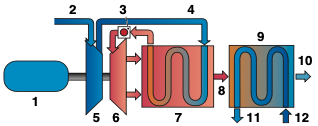
\includegraphics[width=0.49\textwidth]{figs/T100.png}
    \caption{Process flow diagram of a microturbine included as PDF (left) and as PNG (right), to demonstrate the superior quality of PDF over PNG}
    \label{fig:partofpdf}
\end{figure}

\section{Adding annotations on an included picture}
An example of an included picture file (\texttt{JPEG, PNG, \dots}) with annotations added in \LaTeX\ is shown in \cref{fig:valve}. The image of the expansion valve is included with the \cs{includegraphics} command. The dotted CV line, the arrows and symbols are added within \LaTeX\ with simple \TikZ\ drawing commands. Inspect the source file to see how. Another example is shown in \cref{fig:SEM} where a scale is added to an included photo. The properties of the scale (position, color, unit, length, number of ticks) can be customized in the source code.

\begin{frame}{In \TikZ\ you can easily add annotations to included picture files}
    \begin{figure}[b]\centering
    	    \begin{tikzpicture}[scale=0.9]
                \node at (0,0) [above right] {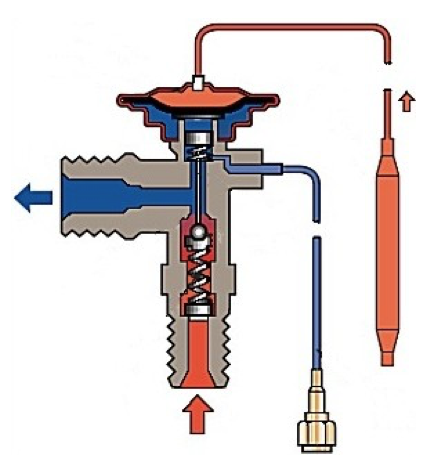
\includegraphics[width=5cm]{figs/expansionvalve}};
    			%\draw [help lines] (-2,-1) grid (8,6); % uncomment to show grid
    			\draw [cv] (2,0) -- (3.5,0) -- ++(0.5,1) -- ++(0,3.5) -- (0,4.5) node[above left] {CV}  -- (0,3) -- cycle;
    			\draw [mass][->] (2.75,-0.5) node [below] {$h_1$} to +(0,0.8);
    			\draw [mass][->] (0.2,3.6)  to  +(-0.7,0) node [left] {$h_2$};
    			\draw [heat][->] (2.7,2)  to [out=230, in=0] (0.5,0.5) node [left] {$\qdot\approx 0$};
    			\draw [work][->] (2.7,3) to (0,2) node [left] {$\wdot=0$};
    			\draw [pin] (4.3,2) -- + (1,-2) node [right,align=left] {pressure\\compensation line};
    			\draw [pin] (5.3,3.5) -- + (1,-2) node [right,align=left] {temperature\\sensor bulb};
			\end{tikzpicture}
    	\caption{Energy flows in a thermostatic expansion valve, to illustrate the addition of annotations in \TikZ}\label{fig:valve}
    \end{figure}
\end{frame}

\begin{figure}\centering
        \begin{tikzpicture}[scale=1]\node at (0,0) [above right] {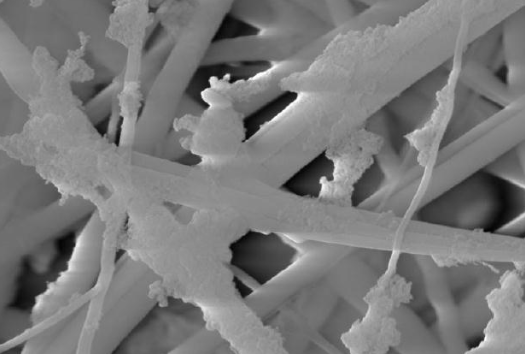
\includegraphics[width=9cm]{figs/SEM}};
            %\draw [help lines] (0,0) grid (8,5); % uncomment to show grid
            \def\scalelength{6cm}           % real length of scale
            \def\nrticks{5}                 % nr of ticks on scale
            \def\scaleunit{\unit{\um}}        % unit on scale
            \coordinate (start) at (1,0.8); % start position of scale
            \begin{scope}[white,thick]      % set color and thickness of scale
                \draw  (start) -- +(\scalelength,0) node [above right] {\scaleunit}; % draw horizontal scale line
                \foreach\tick in {0,1,...,\nrticks}
                {\draw (start) ++(\tick/\nrticks*\scalelength,0) -- +(0,-0.2) node [below] {\tick};} % draw ticks
            \end{scope}
        \end{tikzpicture}
    \caption{SEM image of particles on the fibres of a filter, collected in the flue gas from a biomass boiler, to illustrate the addition of a customized scale with \TikZ}\label{fig:SEM}
\end{figure}

\section{Proper sizing of a figure on a slide}
The aspect ratio of the A4 page format differs from the aspect ratio of a slide in beamer. As a consequence, choosing the proper dimensions of figures, to make them look good on A4 and also on a slide, is sometimes challenging. The trick is to define both the height and width, in combination with the option \verb|keepaspectratio|. It will freeze the aspect ratio of an included picture, to make it fit on A4 and on a slide. Inspect the source code of \cref{fig:radiation} to find out how.

\begin{frame}{The size of this picture depends on the type of document (A4 or slide)}
    \begin{figure}\centering
		     % specifying the height AND the width of an included picture will stretch the picture.
		     % the keepaspectratio option is needed to avoid this.
		     % on A4, the width=0.7\textwidth is the hardest constraint and it will determine the size
		     % with beamer, the height=0.6\textheight is the hardest constraint and it will determine the size
		     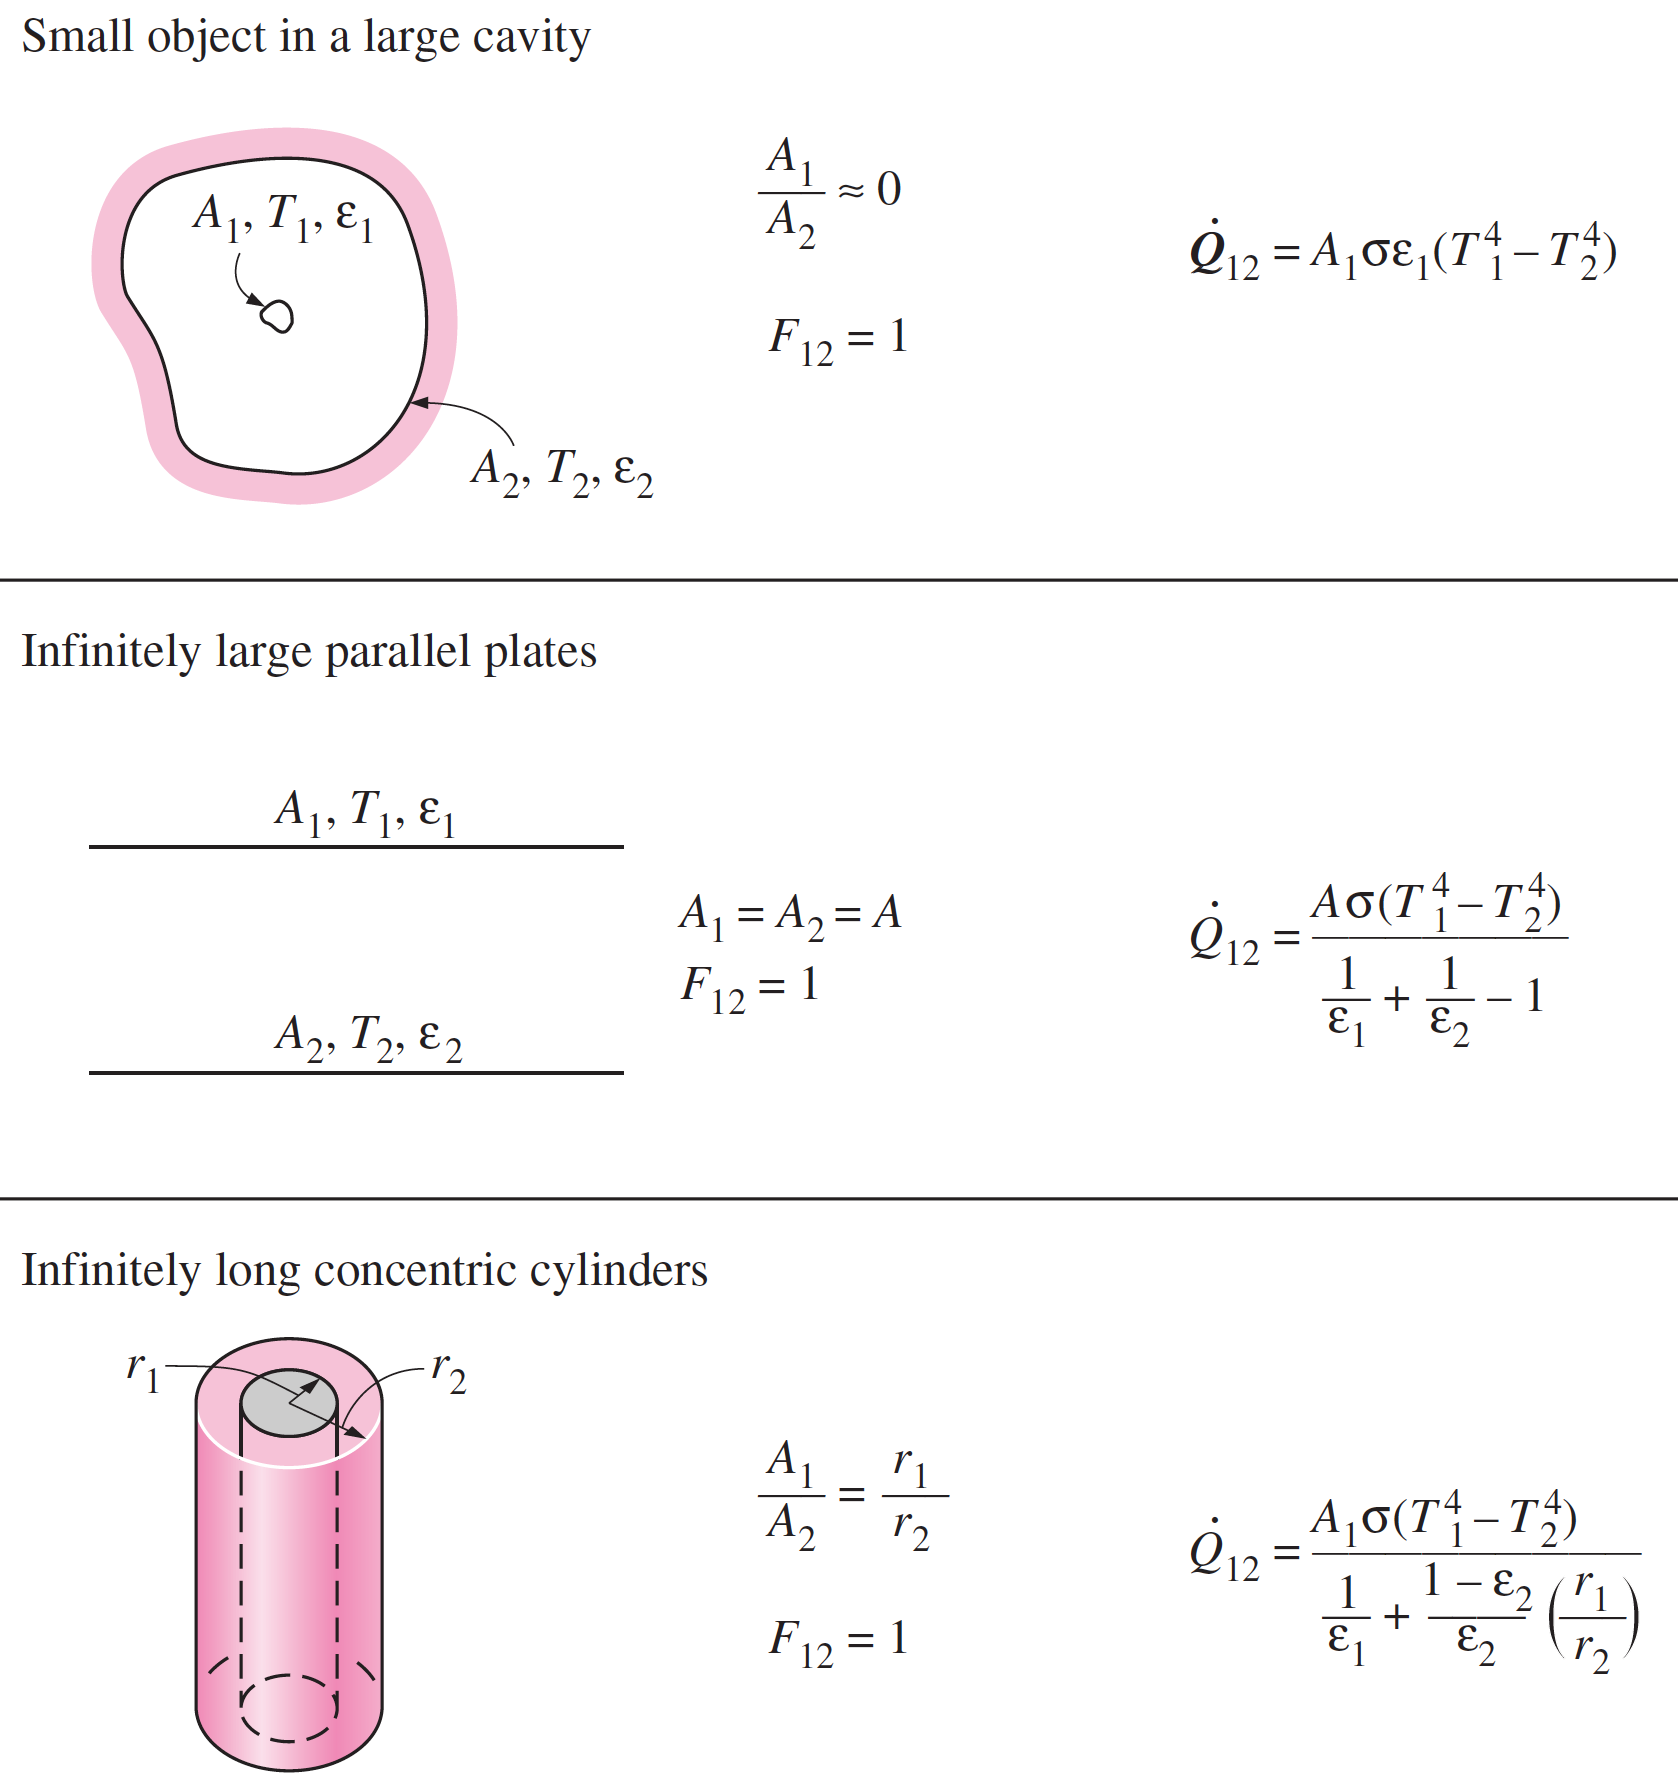
\includegraphics[width=0.7\textwidth,height=0.7\textheight,keepaspectratio]{figs/radiation}
			% 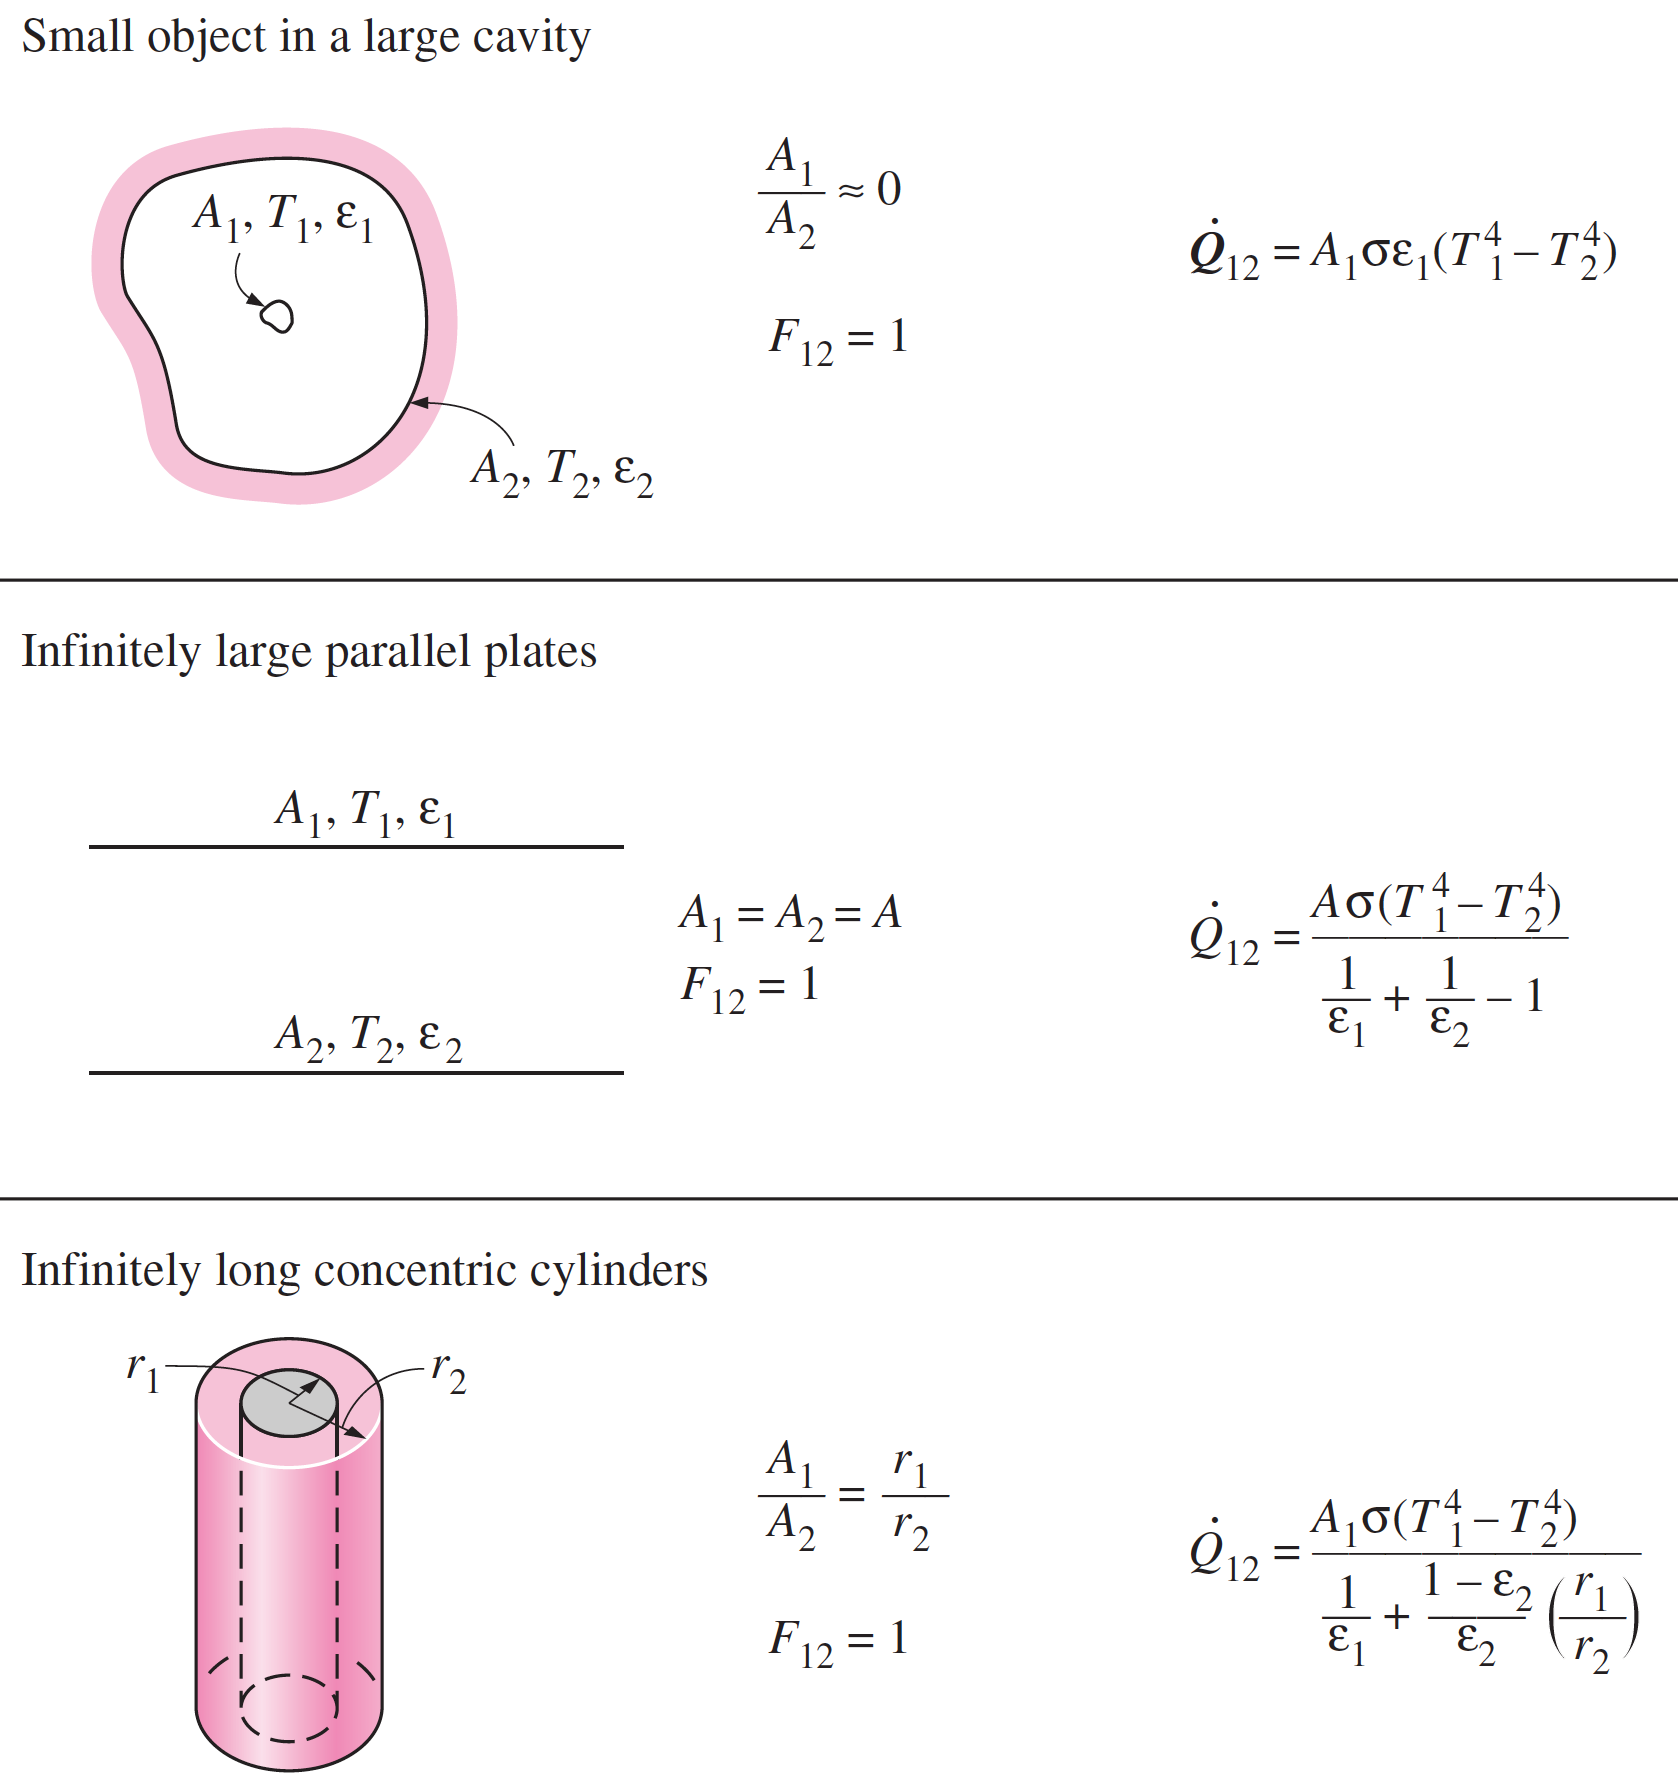
\includegraphics[width=0.8\textwidth,height=0.8\textheight,keepaspectratio]{figs/radiation} % remove comment to see the bad result in beamer: picture too high and caption falls off the slide
			% 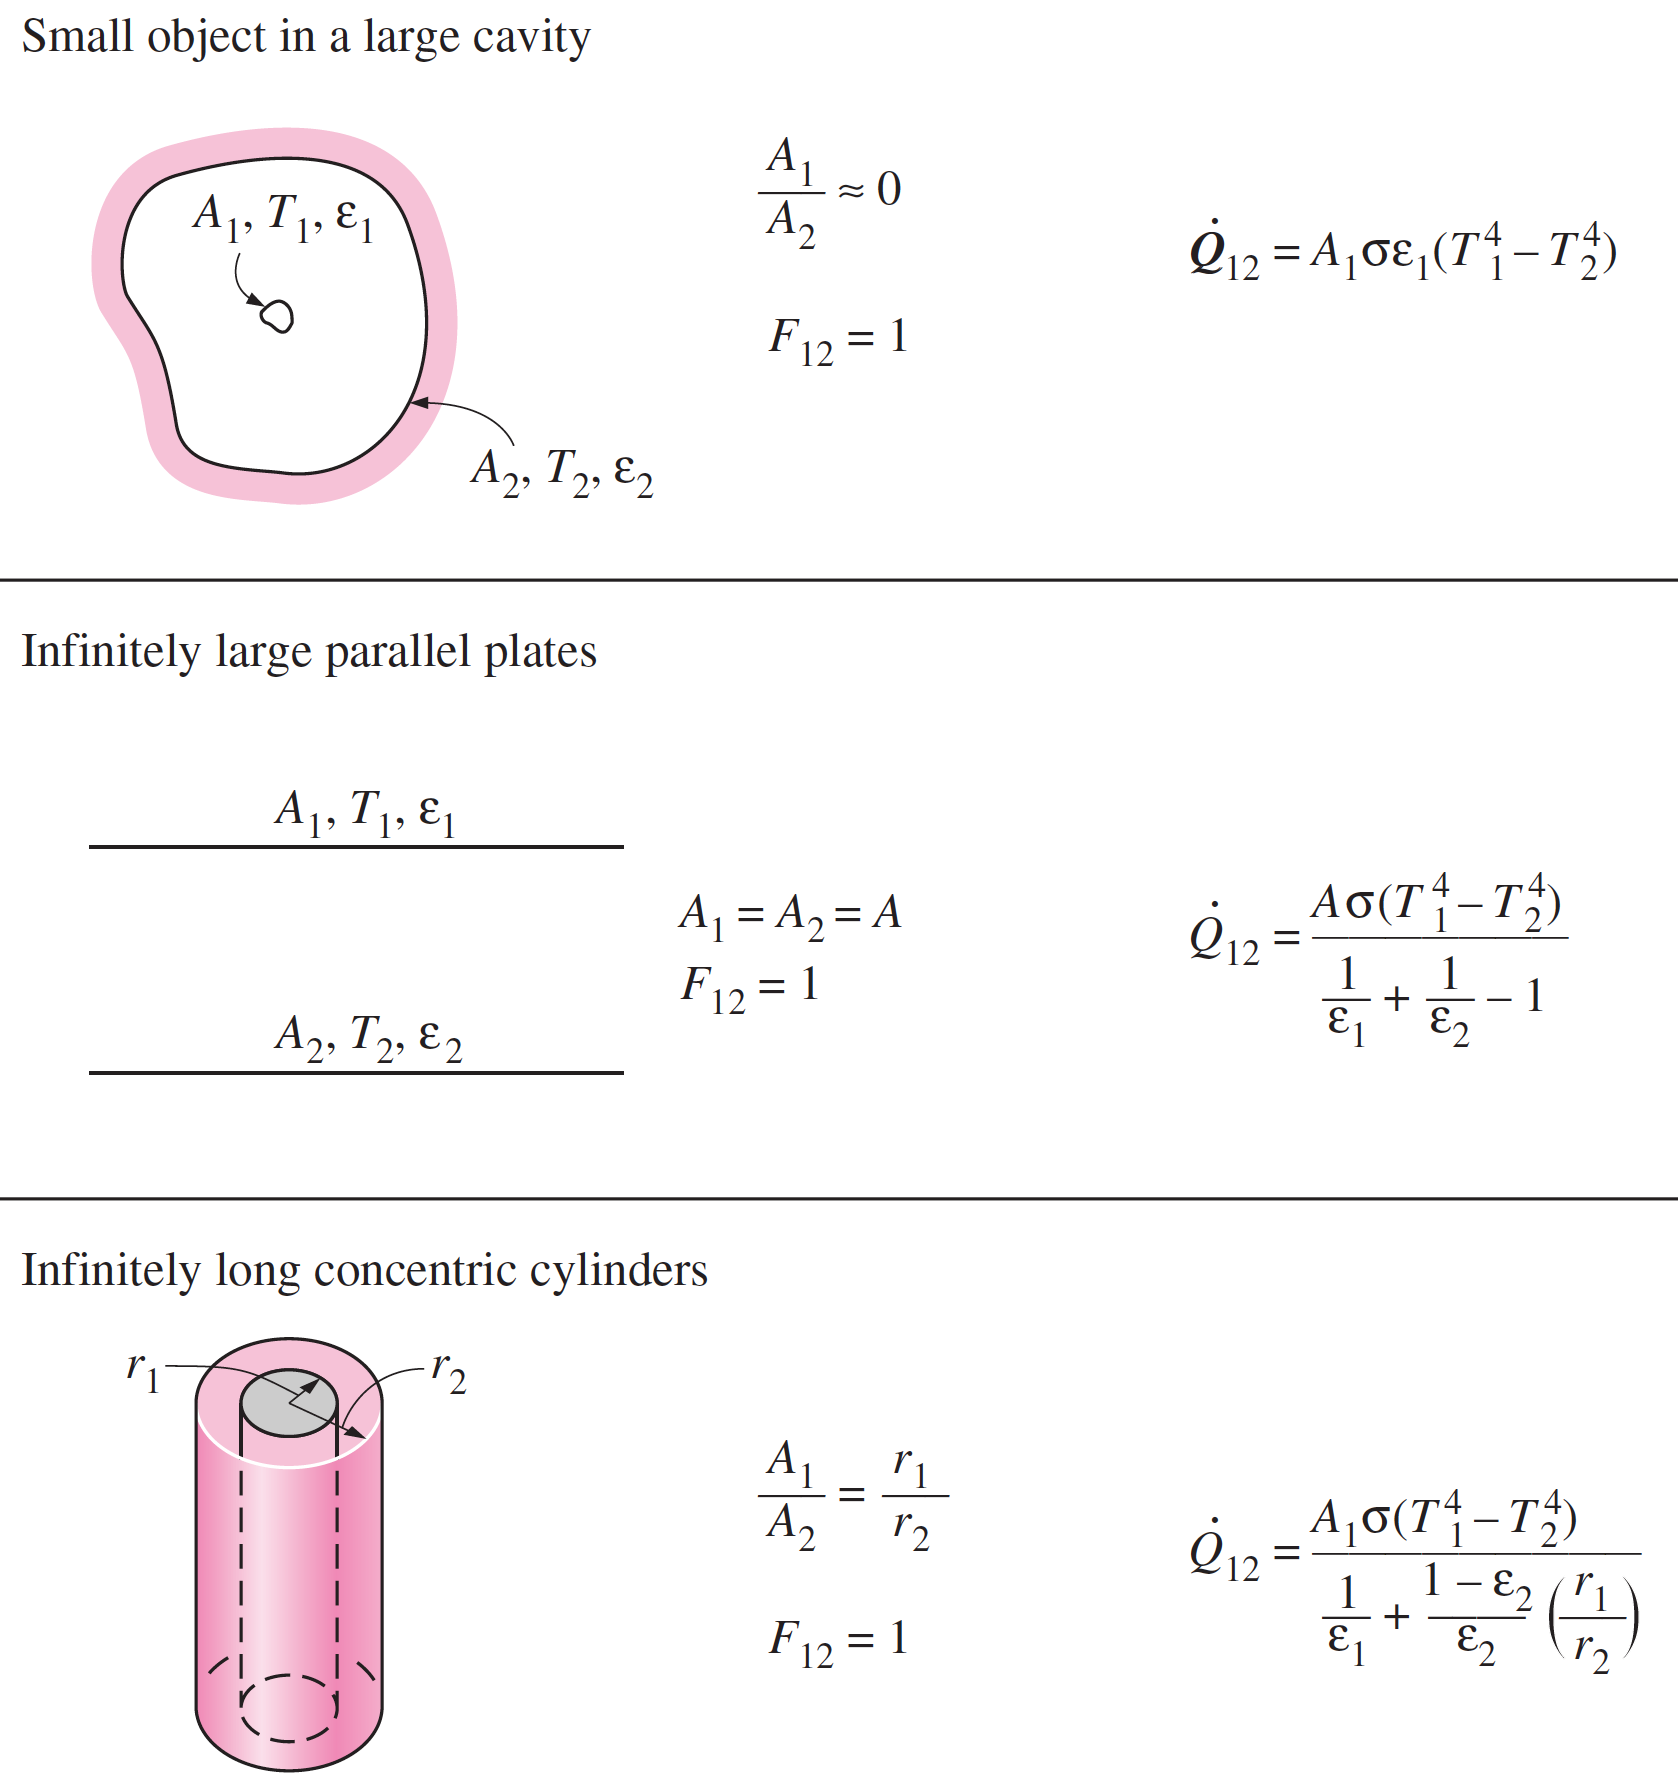
\includegraphics[width=0.8\textwidth,height=0.6\textheight]{figs/radiation} % remove comment to see the stretch
		\caption{Exchange of thermal radiation for some common geometries \parencite{tfs}, to illustrate the use of \texttt{\textbackslash keepaspectratio} to correctly size an included picture file in a manuscript and on a slide}\label{fig:radiation}
    \end{figure}
\end{frame}

\section{Drawing vectors}
Vectors can easily be drawn with \TikZ. See for instance the velocity triangles in a centrifugal pump in  \cref{f:centrifugalpump}. In this drawing, several pump parameters are defined with the command \cs{def}. The goniometric calculations to determine the orientation and magnitude of the velocities are performed with the command \cs{pgfmathsetmacro}. Inspect the source code of the figure in the file \verb|figs/centrifugalpump| for more info. Altering the parameters of the pump will cause the velocity triangles to be automatically recalculated and redrawn.

\begin{figure}\centering
    \begin{tikzpicture}[scale=1]
        % define pump constants, using \def
        \def\rin{1.5}                                   % inner radius
        \def\rout{3.7}                                  % outer radius
        \def\bin{60}                                    % inner beta, degrees
        \def\bout{30}                                   % outer beta, degrees
        \def\bladepos{90}                               % blade position angle, degrees
        \def\bladecurve{60}                             % blade curve angle, degrees
        \def\uin{1.5}                                   % inner rotational velocity
        \def\cin{2.6}                                   % inner absolute velocity
        
        % calculate velocities and angles, using \pgfmathsetmacro for math operations
        \pgfmathsetmacro\uout{\uin*\rout/\rin}          % outer rotational velocity
        \pgfmathsetmacro\coutrad{\cin*\rin/\rout}       % outer absolute radial velocity
        \pgfmathsetmacro\wout{\coutrad/sin{\bout}}      % outer relative velocity
        \pgfmathsetmacro\couttan{\uout-\wout*cos(\bout)}% outer absolute tangential velocity
        \pgfmathsetmacro\tana{\coutrad/\couttan}        % outer absolute tangential velocity
        \pgfmathsetmacro\aout{atan(\tana)}              % outer alpha, degrees
        \pgfmathsetmacro\cout{\coutrad/sin(\aout)}      % outer absolute radial velocity
        
        % draw pump
        \drawcentrifugalpumpcircles{\rin}{\rout}; % draw pump circles
        
        % draw blade
        {\drawcentrifugalpumpblade{\rin}{\rout}{\bladepos}{\bladecurve}{\bin}{\bout}};
 
        % draw velocity triangle at inlet
        \draw [rotation,->] (root) -- +(0:\uin) node [right] {$u_1$};
        \draw [absolute,->] (root) -- +(90:\cin) node [right] {$c_1=c_\up{1r}$};
        \draw [relative,->] (root) -- +(-\uin,\cin) node [right] {$w_1$};
        
        % draw velocity triangle at outlet
        \draw [rotation,->] (tip) -- +(\bladecurve:\uout) coordinate (U2) node [left] {$u_2$};
        \draw [relative,->] (tip) -- +(180+\bladecurve-\bout:\wout) coordinate (W2) node [left] {$w_2$};
        \draw [absolute,->] (tip) -- +(90+\bladecurve:\coutrad) node [left] {$c_\up{2r}$};
        \coordinate (C2) at ($(U2)   +({180+\bladecurve-\bout}:{\wout})$);
        \draw [absolute,->] (tip) -- (C2) node [right] {$c_\up{2}$};
        \draw [axis] (W2) -- (C2);  % connect end of w2, c2r, c2
        
        % draw angles: location, angle1, angle2, label, arc radius, label pos, left/right
        \drawangle{root}{180}{180-\bin}{$\beta_1$}{0.4cm}{0.5}{left};                         % beta 1
        \drawangle{tip}{180+\bladecurve}{180+\bladecurve-\bout}{$\beta_2$}{1cm}{0.1}{left};   % beta 2
        \drawangle{root}{0}{90}{$\alpha_1$}{0.4cm}{0.5}{right};                               % alpha 1
        \drawangle{tip}{\bladecurve}{\bladecurve +\aout}{$\alpha_2$}{1cm}{0.4}{above}         % alpha 2
\end{tikzpicture}



    \caption{Velocity triangles at the root (1) and tip (2) of a impeller blade in a centrifugal pump, to illustrate the drawing of vectors and angles in \TikZ}\label{f:centrifugalpump}
\end{figure}

\section{Drawing free-body diagrams}
An example of a mechanical sketch of two bodies on a slope connected with a wire and the related free-body diagrams are shown in \cref{fig:freebody}. The original \TikZ\ code was written by \cite{freebody} and can be found on \href{http://www.texample.net/tikz/examples/free-body-diagrams}{TeXample net}. Drawings in \TikZ\ can be parametric. In this case, the inclination angle of the slope can be altered by changing the value in the definition \verb|\def\iangle{45}| in the source code. The angle in \cref{fig:freebody} is \ang{45} while the angle in the original drawing was \ang{30}.

\begin{frame}{Drawings and diagrams can be parameterized and synchronized,\\ check the source code to see how}
    \begin{figure}[htb]\centering
        \input{figs/freebody.tex} % source: http://www.texample.net/tikz/examples/free-body-diagrams
        \caption{A mechanical sketch and two corresponding free-body diagrams made with \TikZ\ \parencite[adapted from][]{freebody}, to illustrate the use of parameters in drawings}\label{fig:freebody}
    \end{figure}
\end{frame}

\section{Drawings with a 3D look}
Drawings that create a 3D look, are also easy to make, as shown in \cref{fig:torque}.

\begin{frame}{You can easily add math expressions to drawings}
    \begin{figure}\centering
        \begin{tikzpicture}[scale=0.7]
            % \draw [helpline] (-2,-2) grid (5,5);
            \draw[fill=blue!20](0,0) circle (1 and 2);
            \draw[top color=blue!10,bottom color=black!70,middle color=blue!30] (-0.5,2) arc (90:270:1 and 2) -- ++(0.5,0) arc (-90:-270:1 and 2) -- cycle;
            \draw[top color=white,bottom color=black!70] (0,3mm) arc (90:270:1.5mm and 3mm)--++(2cm,0) arc (-90:-270:1.5mm and 3mm)-- cycle;
            \draw (2cm,3mm) arc (90:-90:1.5mm and 3mm);
            \draw[->] (1.5,0.4) arc (55:325:0.2cm and 0.6cm) node[pos=0.8, below] {$\omega$};
            \draw[measure,->] (0,0) --  ++(155:1.4) node[midway, above] {$\vec{r}$};
            \draw[force,->] (0,0) ++(155:1.4) --  ++(255:2.5) node[near end, left] {$\vec{F}$};
            \draw[torque,->] (0,0) -- ++(3,0) node[right,align=left] {$\vec{T}=\vec{r}\times \vec{F}$};
            \node at (6,1.5) [right] {$W_\up{shaft}=T\,\Delta\theta\units{J}$};
            \node at (6,0.5) [right] {$\wdot_\up{shaft}= T\,\omega=T\, \frac{2\pi N}{60}\units{W}$};
            \node at (6,-0.5) [right] {$T$};
            \node at (6,-1.5) [right]  {$\Delta\theta$};
            \node at (6,-2.5) [right] {$N$};
            \node at (7,-0.5) [right] {torque [Nm]};
            \node at (7,-1.5) [right]  {rotation angle [rad]};
            \node at (7,-2.5) [right] {rotational speed [rpm]};
        \end{tikzpicture}
    	\caption{Transfer of mechanical power with a shaft, to illustrate the capacity of \TikZ\ to make 3D drawings}\label{fig:torque}
    \end{figure}
\end{frame}

\section{Plotting airfoils}
The Applied Aerodynamics Group of the university of Illinois has an online database of more than 1600 airfoils \citep{airfoils}. The airfoil data is made available in data files with the extension \verb|.dat|. Data files can be plotted directly in \LaTeX\ if the headers are removed. See \cref{fig:airfoil} where the \href{https://m-selig.ae.illinois.edu/ads/coord/e625.dat}{Eppler 625 airfoil data} is plotted, combined with a grid.

\begin{frame}{It is possible to plot data straight from a DAT-file}
	\begin{figure}[b]\centering
        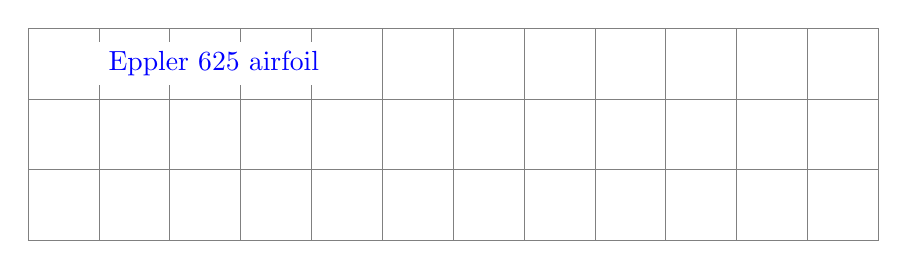
\begin{tikzpicture}[scale=0.9]
        \draw [help lines] (-1,-1) grid (11,2);
        \draw [scale=10,blue,very thick] plot file{data/e625profile.dat};
        \node [blue,fill=white,right] at (0,1.5) {Eppler 625 airfoil};
        \end{tikzpicture}
		\caption{A plot of an Eppler 625 airfoil with \TikZ\ \parencite[data from][]{airfoils}, to illustrate the plotting of data from a DAT-file}\label{fig:airfoil}
	\end{figure}
\end{frame}

\section{Repeating patterns}
Technical and scientific drawings often contain repeating patterns. The command \texttt{\textbackslash foreach} can be used to repeat drawing commands, to create patterns like for instance the pattern of tubes in \cref{fig:pattern}. The number of rows and layers of tubes can easily be adapted in the source code. Other examples can be found in the \href{https://tikz.dev/pgffor}{Pgf/\TikZ\ manual}.

\begin{frame}{Repeating patterns can easily be plotted in \TikZ}
	\begin{figure}\centering
        \def\hxwidth{8cm}      % heat exchanger width
        \def\hxheight{6cm}     % heat exchanger height
        \def\nrrows{4}         % nr of tube rows
        \def\nrlayers{7}       % nr of tube layers
        \begin{tikzpicture}
            %\draw [helpline] (0,0) grid (5,5);
            \draw [process]    (0,0)         -- + (\hxwidth,0); % bottom plate
            \draw [process]    (0,\hxheight) -- + (\hxwidth,0); % top plate
            \draw [mass,->]    (-1,\hxheight/2) node [left] {$\mdot_\up{air}$} -- + (1,0) ; % mass flow in
            \draw [measure,<->](\hxwidth-0.3cm,0) -- node [right] {$H$} + (0,\hxheight) ; % height of channel
            \foreach \row   in {1,2,...,\nrrows}
            \foreach \layer in {1,2,...,\nrlayers}
            {\node[circle, draw, minimum size=0.4cm] (\row\layer) at ({\layer/\nrlayers*(\hxwidth-1cm)},{\row/\nrrows*(\hxheight-1cm)}){};}
            \draw [measure,<->] (11.east)  -- node [below]{$d_1$} (12.west);
            \draw [measure,<->] (12.north) -- node [right]{$d_2$} (22.south);
        \end{tikzpicture}
		\caption{A cross-flow heat exchanger with the pipes arranged in \nrrows\ rows and \nrlayers\ layers, to illustrate the use of \cs{foreach} in \TikZ\ to draw patterns}\label{fig:pattern}
	\end{figure}
\end{frame}

\section{Plotting analytical functions}
It's also easy to plot analytical functions as shown in \cref{fig:analyticalfunctions}. In this example, three analytical functions are plotted. Inspect the source code to see the various plot settings, such as the domain, the minimum and maximum values on the axes, the size of the plot, the legend and line styles.

\begin{figure}[htb]\centering
    \def\funA{6*x*x-20*x+10} % definition of function A
        \begin{tikzpicture}
            \begin{axis}[
             width =0.9\linewidth,    % scale the width
             height=0.35\textheight,   % scale the height
             xmin=-6.28,
             xmax=6.28,
             xlabel= $x$,
		     ylabel= $y$,
             samples=200,
             legend pos= north east,
             legend cell align=left,
             ]
            \addplot[teal,domain=1:5,ultra thin](x,{\funA}); % braces needed to protect
            \addlegendentry{$y=6x^2-20x+10$};
            \addplot[blue,dashed,domain=-6:0.5](x,{30*sin(deg(3*x))-100}); % braces needed to protect
            \addlegendentry{$y=30\sin 3x - 100$};
            \addplot[magenta, thick]({0.2*x*x*x},-40*x); % braces needed to protect
            \addlegendentry{$x=f(y) \rightarrow$ see source code};
            \end{axis}
        \end{tikzpicture}
	\caption{Plot of three analytical functions, to illustrate various types of plot settings in \TikZ}\label{fig:analyticalfunctions}
\end{figure}

\section{Plotting random data}

\begin{figure}\centering
    \begin{tikzpicture}
        \def\spacing{5.2cm}
        \begin{scope}[shift={(0,0)}]
            \drawtarget{precise and accurate};
            \drawshots{0}{0.2};   % position, spread
        \end{scope}
        \begin{scope}[shift={(\spacing,0)}]
            \drawtarget{precise but not accurate};
            \drawshots{1.5}{0.2}; % position, spread
        \end{scope}
        \begin{scope}[shift={(0,-\spacing)}]
            \drawtarget{not precise but accurate};
            \drawshots{0}{0.7};   % position, spread
        \end{scope}
        \begin{scope}[shift={(\spacing,-\spacing)}]
            \drawtarget{not precise and neither accurate};
            \drawshots{1.5}{0.7}; % position, spread
        \end{scope}
    \end{tikzpicture}
    \caption{Four combinations of accuracy and precision, to illustrate the plotting of random data in \TikZ, adapted from \href{https://tex.stackexchange.com/questions/449894/how-to-make-accuracy-precision-graphic}{StackExchange}}\label{fig:randomdata}
\end{figure}


\section{Plotting experimental data against a model}
It is also possible to combine analytic functions with experimentally obtained data in a single plot, with inclusion of the measurement errors. This is shown in \cref{fig:psat} where experimental data is plotted against a simple parabolic model.

\begin{figure}\centering
	\begin{tikzpicture}[scale=1]
		\begin{axis}[
        width =0.90\linewidth,    % scale the width
        height=0.35\textheight,   % scale the height
		xlabel=$T\ \unitschart{\celsius}$,
		ylabel= $\psat\unitschart{kPa}$,
		ylabel near ticks,
		legend pos= north west,
		legend cell align=left,
		]
		\addplot[blue,domain=0:50,samples=100]{0.004*x^2+1};
        \addlegendentry{$\psat=0.004\cdot T^2+1$ (model)}
		\addplot[brown,only marks, mark=x,error bars/y dir =both,error bars/y fixed = 1] coordinates {
			(0,0.61) (5,0.87) (10,1.23) (15,1.71) (20,2.34) (25,3.17) (30,4.25) (35,5.6286) (40,7.39) (45,9.5944) (50,12.352)};
			\addlegendentry{measurements};
		\end{axis}
	\end{tikzpicture}
	\caption{The saturation pressure of water as function of temperature, to demonstrate the plotting of model data against experimental data with error bars}\label{fig:psat}
\end{figure}

\section{Predefined plot settings}
It's also possible to predefine the settings of axes. See for instance the definition of \verb|axespsychro| in the style file \verb|styles/myDrawingStuff| and how easy it is to use it as an option in: \\\verb|\begin{axis}[axespsychro]| in the source code of \cref{fig:psychrochart} and \cref{fig:psychrochart2}. Both charts have exactly the same appearance because of the same predefined settings.

\begin{figure}\centering
		\begin{tikzpicture}[scale=1.0]
    		\begin{axis}[axespsychro]
            \drawsaturationline{sat};
            \coordinate (A) at (axis cs: 30,10);
            \coordinate (B) at (axis cs: 19.2,14.3);
            \coordinate (C) at (axis cs: 13.5,10);
            \draw [process,deco=0.6] (A) -- (B) node [above left] {$T_\up{WB}$};  
            \draw [process,deco=0.6] (A) -- (C) node [above left] {$T_\up{DP}$}; 
            \draw [helpline] (A) -- (axis cs:30,0) node [above right] {$T_\up{DB}$}; 
            \draw [helpline] (A) -- (axis cs:50,10); % 
            \drawdot{A};\drawdot{B};\drawdot{C};
    		\end{axis}
		\end{tikzpicture}
		\caption{A simplified psychrometric chart with indication of the dew point and the wet bulb temperature of humid air, to illustrate the use of predefined plot settings}\label{fig:psychrochart}
\end{figure}

\begin{figure}\centering
		\begin{tikzpicture}[scale=1.0]
			\begin{axis}[axespsychro]
            \drawsaturationline{sat};
            \coordinate (A) at (axis cs: 40,5);
            \coordinate (B) at (axis cs: 4.5,5);
            \draw [process,deco=0.5] (A) -- (B) node [above left] {$T_\up{DP}$}; % 
            \draw [helpline] (A) -- (axis cs: 40,0); % 
            \draw [helpline] (A) -- (axis cs: 50,5); % 
            \drawdot{A};\drawdot{B};
			\end{axis}
		\end{tikzpicture}
		\caption{A simplified psychrometric chart with indication of the dew point of humid air, to illustrate the use of the same predefined plot settings as in \cref{fig:psychrochart}}\label{fig:psychrochart2}
\end{figure}

\section{Grouping of plots}
Plots can be grouped in such a way that they share the same $x$-axis and/or $y$-axis. An example where both axes are shared is shown in \cref{fig:groupplot}.

\begin{frame}{A group plot will resize itself to the aspect ratio of the slide}
	\begin{figure}\centering
		\begin{tikzpicture}\tinybeamer
	\begin{groupplot}[group style={group size=2 by 2,vertical sep=1em,horizontal sep=2ex,x descriptions at=edge bottom,y descriptions at=edge left},
	xmin=-2.7,xmax = 11.2,ymin=0,ymax=100,
	xlabel={$\qdot_\up{exchanged}\unitschart{kW}$},
	ylabel= {$T\unitschart{\SI{}{\celsius}}$},
	height=0.45\textheight,width=0.55\textwidth]
    	\nextgroupplot	\def\Q{1.3}; % Q in kW
    	\draw [blue,deco=0.5] (axis cs: 0,20) -- (axis cs: \Q,20+\Q/0.2/1) node [right] {\SI{26}{\celsius}};
    	\draw [red,deco=0.5](axis cs: \Q,90)  -- (axis cs: 0,90-\Q/0.03/4.18)  node [left] {\SI{80}{\celsius}};
    	\draw[helpline] (axis cs: 0,90-\Q/0.03/4.18) -- (0,0) (\Q,0) -- (\Q,90);
    	\draw[measure,<->] (axis cs: 0,10) -- (axis cs: \Q,10) node [right]{\Q~kW};
    	\node at (axis cs: 5,70) [right,align=left]{$A=\SI{0.68}{m^2}$};
    	\nextgroupplot \def\Q{2.5}; % Q in kW
    	\draw [blue,deco=0.5] (axis cs: 0,20) -- (axis cs: \Q,20+\Q/0.2/1) node [right] {\SI{33}{\celsius}};
    	\draw [red,deco=0.5](axis cs: \Q,90)  -- (axis cs: 0,90-\Q/0.03/4.18)  node [left] {\SI{70}{\celsius}};
    	\draw[helpline] (axis cs: 0,90-\Q/0.03/4.18) -- (0,0) (\Q,0) -- (\Q,90);
    	\draw[measure,<->] (axis cs: 0,10) -- (axis cs: \Q,10) node [right]{\Q~kW};
    	\node at (axis cs: 5,70) [right,align=left]{$A=\SI{1.6}{m^2}$};
    	\nextgroupplot \def\Q{3.8}; % Q in kW
    	\draw [blue,deco=0.5] (axis cs: 0,20) -- (axis cs: \Q,20+\Q/0.2/1) node [right] {\SI{39}{\celsius}};
    	\draw [red,deco=0.5](axis cs: \Q,90)  -- (axis cs: 0,90-\Q/0.03/4.18)  node [left] {\SI{60}{\celsius}};
    	\draw[helpline] (axis cs: 0,90-\Q/0.03/4.18) -- (0,0) (\Q,0) -- (\Q,90);
    	\draw[measure,<->] (axis cs: 0,10) -- node [above]{\Q~kW} (axis cs: \Q,10);
    	\node at (axis cs: 5,70) [right,align=left]{$A=\SI{2.8}{m^2}$};
    	\nextgroupplot \def\Q{8.8}; % Q in kW
    	\draw [blue,deco=0.5] (axis cs: 0,20) -- (axis cs: \Q,20+\Q/0.2/1)  node [right] {\SI{64}{\celsius}};
    	\draw [red,deco=0.5](axis cs: \Q,90) -- (axis cs: 0,90-\Q/0.03/4.18) node [left] {\SI{20}{\celsius}};
    	\draw[helpline] (axis cs: 0,90-\Q/0.03/4.18) -- (0,0) (\Q,0) -- (\Q,90);  
    	\draw[measure,<->] (axis cs: 0,10) -- node [above]{\Q~kW $=\qdot_\up{max}$} (axis cs: \Q,10); 
    	\node at (axis cs: -2,70) [right,align=left]{$A=\infty~\up{m^2}$};
	\end{groupplot}
\end{tikzpicture} % if the code for a drawing is long, put it in a separate file
		\caption{The effect of heat exchanger surface on heat exchanger duty, to illustrate the use of shared axes in group plots}\label{fig:groupplot}
	\end{figure}
\end{frame}

\section{Plotting data from an external file}
Data can also be read from external files and then plotted, as in \cref{fig:thermalpower} and \cref{fig:CO2}. Even if the data in the file contains date- and timestamps (like for instance of the type \texttt{YYYY-MM-DD HH:MM}) they can still be plotted by using the \TikZ\ library \texttt{dateplot}. An example of such a plot is shown in \cref{fig:weatherdata}. The weather data was fetched from \cite{mesonet}, an ever-growing archive of automated airport weather observations from around the world.

\begin{figure}\centering
    \begin{tikzpicture}[scale=1]
      \begin{axis}[
          width =1.00\linewidth,    % scale the width
          height=0.40\textheight,   % scale the height
          grid=major, 
          grid style={dashed,gray!15},
          xlabel={Time}, % Set the labels
          ylabel={Thermal power},
          x unit=\unit{\hour}, % Set the respective units
          y unit=\unit{\kW}, % Set the respective units
          legend pos= north east,
          ]
          \addplot[cyan,mark=*,mark size=1pt] table[x index=0, y index=1,col sep=comma] {data/thermal.csv}; % read data from file
          \legend{building}
      \end{axis}
    \end{tikzpicture}
    \caption{Thermal power demand for a building during one week, to illustrate the plotting of time series data from a csv-file}\label{fig:thermalpower}
\end{figure}

\begin{figure}\centering
    \begin{tikzpicture}[scale=1]
      \begin{axis}[
          width =1.00\linewidth,    % scale the width
          height=0.40\textheight,   % scale the height
          grid=major, 
          grid style={dashed,gray!15},
          xmax=230,
          ymax=6,
          xlabel={Emissions}, % Set the labels
          ylabel={Payback time},
          x unit={kg\ch{CO2}eq/year}, % Set the respective units
          y unit={year}, % Set the respective units
          legend pos= north east,
          ]
          \addplot[brown,mark=triangle,mark size=2pt,only marks] table[x index=0, y index=1,col sep=comma] {data/CO2.csv}; % read data from file
          \draw [blue] plot[smooth, tension=0.5] coordinates {(80,6) (81,4) (92,3) (120,2.5) (180,2.15) (223,1.95)}; % draw pareto front
          \node[pin, rotate=-40] at (90,2.85) {Pareto front}; % place text
      \end{axis}
    \end{tikzpicture}
    \caption{The payback time and the \ch{CO2} emissions for different configurations of a solar panel installation, to illustrate the creation of scatter plots from data on a csv-file}\label{fig:CO2}
\end{figure}

\begin{figure}\centering
    \begin{tikzpicture}[scale=1]
      \begin{axis}[
        width =1.00\linewidth,    % scale the width
        height=0.95\textheight,   % scale the height
        grid=major, 
        grid style={dashed,gray!30}, % this grid is a bit more dark
        date coordinates in=x, % to indicate that the dates are in x-axis
        %xmin=2020-03-01 00:00,
        %xmax=2020-03-07 23:59,
        xtick distance=1, % set `xtick distance' to 24 hours (24/24)
        % xtick=data, % to use every entry as xtick
        xticklabel={\day-\month},
        xlabel={April 2020},
        ylabel={Temperature},
        y unit=\unit{\celsius}, % Set the respective units
        legend pos=south east, % to place the legend
        legend cell align=left, % to align the text in the legend
        ]
        \addplot [red] table [col sep=comma,x index=1, y index=2] {data/weather.csv};
        \addplot [blue] table [col sep=comma,x index=1, y index=3] {data/weather.csv};
        \legend{dry bulb temperature, dew point}
      \end{axis}
    \end{tikzpicture}
    \caption{Weather data for Brookneal Virginia (USA) in the first week of April '20, to illustrate the sizing of plots, here the plot is sized to fill the entire  page}\label{fig:weatherdata}
\end{figure}

% more info on \mode<all> in section 21.3 of beameruserfile.pdf
\mode<all>
